\documentclass[12pt]{article}
\usepackage{enumitem}
%\usepackage[T1]{fontenc}
\usepackage[auth-sc,affil-sl]{authblk}
\usepackage{amsmath}
\usepackage{graphicx}
\usepackage{color}
%\usepackage{enumerate}
\usepackage[round]{natbib}
%\usepackage{url} % not crucial - just used below for the URL 
%\usepackage{amsthm}
\usepackage{amssymb}
\usepackage{graphicx}
\usepackage{epstopdf}
\usepackage{hyperref}
\usepackage{alltt}
\usepackage{listings}
\usepackage{array}
\usepackage[noline, boxed, linesnumbered, procnumbered, titlenumbered]{algorithm2e}
\usepackage[firstpage]{draftwatermark}
\usepackage[margin=1in]{geometry}  %%jcgs has own margins
\usepackage{lmodern}

%\pdfminorversion=4
% NOTE: To produce blinded version, replace "0" with "1" below.
\newcommand{\blind}{0}

\newcommand{\secref}[1]{Section~\ref{#1}}
\newcommand{\tblref}[1]{Table~\ref{#1}}
\newcommand{\figref}[1]{Figure~\ref{#1}}
\newcommand{\thmref}[1]{Theorem~\ref{#1}}
\newcommand{\algref}[1]{Algorithm~\ref{#1}}
\newcommand{\funref}[1]{Function~\ref{#1}}
\newcommand{\listingref}[1]{Listing~\ref{#1}}

\newcommand{\eg}{{\em e.g.}}
\newcommand{\ith}{$i^{th}$}
\newcommand{\cut}[1]{}
\newcommand{\todo}[1]{{\bf\em TODO:} {{#1}}}

\newcommand{\spd}{\fontfamily{cmr}\textsc{\small StratPD}}
\newcommand{\cspd}{\fontfamily{cmr}\textsc{\small CatStratPD}}

\setlist[enumerate]{itemsep=-1mm}

% DON'T change margins - should be 1 inch all around.
\cut{
\addtolength{\oddsidemargin}{-.5in}%
\addtolength{\evensidemargin}{-.5in}%
\addtolength{\textwidth}{1in}%
\addtolength{\textheight}{1.3in}%
\addtolength{\topmargin}{-.8in}%
}

\begin{document}

\def\spacingset#1{\renewcommand{\baselinestretch}%
{#1}\small\normalsize} \spacingset{1}


%%%%%%%%%%%%%%%%%%%%%%%%%%%%%%%%%%%%%%%%%%%%%%%%%%%%%%%%%%%%%%%%%%%%%%%%%%%%%%

\if0\blind
{
  \title{{\fontfamily{cmr}\textsc{StratPD}}: \bf A Localized Approach to Partial Dependence Plots for Codependent Variables}

  \author{Terence Parr and James Wilson\\
      University of San Francisco\\
}
  \maketitle
} \fi

\if1\blind
{
  \bigskip
  \bigskip
  \bigskip
  \begin{center}
    {\LARGE\bf Title}
\end{center}
  \medskip
} \fi

\bigskip
\begin{abstract}
Pithy abstract here.
\end{abstract}

\noindent%
{\it Keywords:} beer, bbq
%\vfill

%\newpage
%\spacingset{1.5} % DON'T change the spacing!
\section{Introduction}
\label{sec:intro}

In practice, machine learning model interpretation is just as important as obtaining an accurate model. Feature importance is one such interpretation tool, which indicates the relative predictive power of each feature and is helpful when making business decisions. For example, in a model predicting apartment rent prices, the important features often identify what renters are willing to pay for. On the other hand, feature importance does not identify the relationship itself between features (explanatory variables),  and the target (response) variable.  Knowing these relationships tells model users a great deal about their data and, indirectly, the associated real-world population. For example, public health officials might be interested in how years of education affect body weight, given a set of observations sampled from a population.

Given just one or two features, a plot of any feature versus the target lets us visualize the exact relationship, this approach does not work for data sets with more than two features because we cannot visualize more than three dimensions.

To get around this limitation, traditional marginal plots project other axes onto the plane associated with the feature of interest and target variable.  That means that marginal plots do not isolate the specific contribution of a feature of interest to the target. For example, a marginal plot of sex (male/female) versus body weight would likely show that, on average, men are heavier than women. While true, men are also taller than women on average, which likely accounts for most of the difference in average weight. It's unlikely that two ``identical'' people, differing only in sex, would be appreciably different in weight.  

\cite{PDP} introduced partial dependence (PD) plots as a way to extract and visualize the dependence of the target on one or two features of interest.  Consider a New York City apartment rent data set from Kaggle \cite{rent-dataset} and the marginal plot in \figref{fig:baths_price}(a) showing the number of bathrooms versus price.  \figref{fig:baths_price}(b) shows the (zero-centered) PD of rent price on the number of bathrooms as a black line. The partial dependence line is the average of the blue lines, which represent the individual conditional expectation (ICE) plots of \cite{ICE}.  In this case, the ICE lines depict the model prediction contributions for a single observation as the bathroom feature shifts through all possible number of bathrooms. Because PD plots represent an average across observations, they can hide a great deal of variability, so it is helpful to combine PD and ICE plots.

\begin{figure}[htbp]
\begin{center}
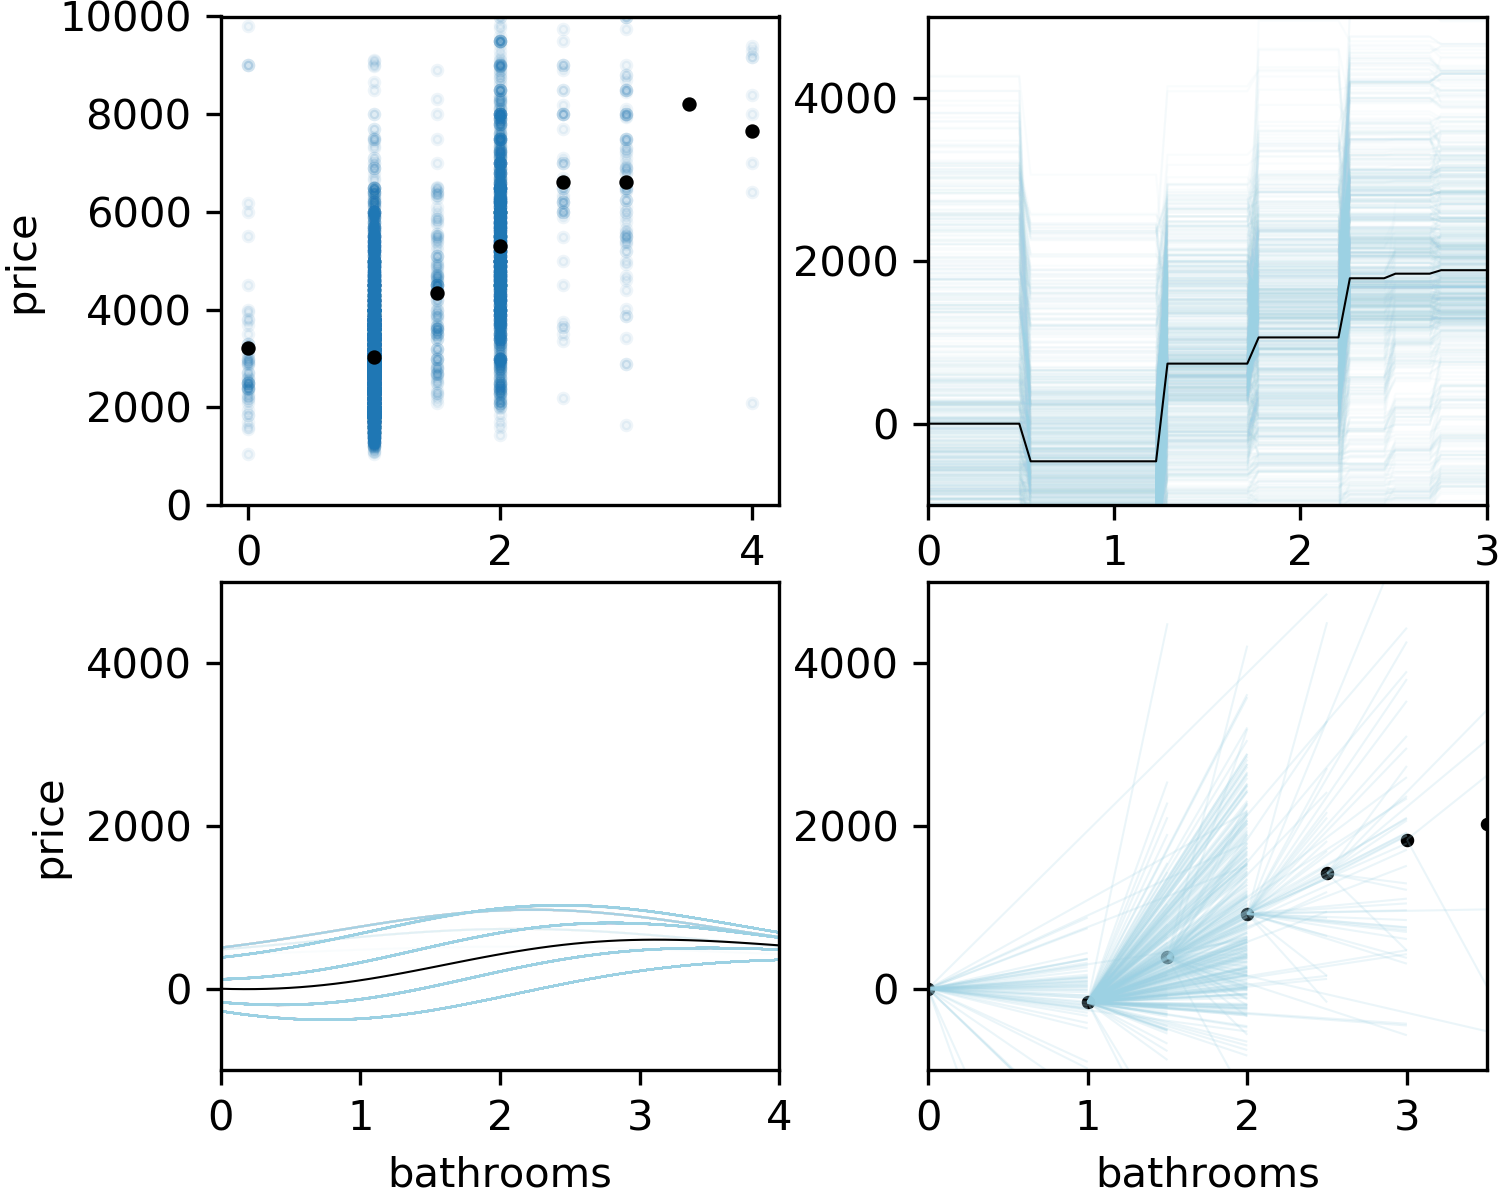
\includegraphics[scale=0.7]{images/bathrooms_vs_price.png}
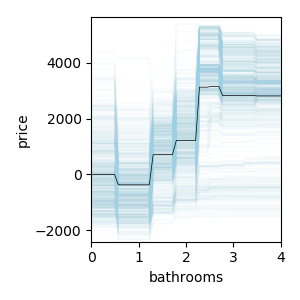
\includegraphics[scale=0.7]{images/bathrooms_vs_price_pdp.png}\\
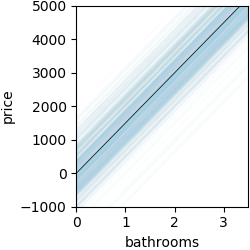
\includegraphics[scale=0.7]{images/bathrooms_vs_price_pdp_lm.png}
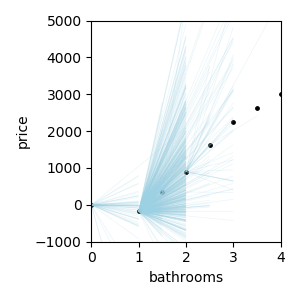
\includegraphics[scale=0.7]{images/bathrooms_vs_price_stratpd.png}
\caption{{\bf  Marginal plot, PDP/ICE plot, and \spd{} plot of bathrooms versus rent price; sample size 9000 of 400k...}}
\label{fig:baths_price}
\end{center}
\end{figure}

\cut{The partial dependence plot broadly follows the marginal plot except for the prices of two and three bathroom apartments, where it levels off. This is counterintuitive and exposes an issue with PD and ICE plots.} While PD and ICE plots are {\em model-agnostic}, they are not {\em model-independent} and are subject to the strengths and weaknesses of the model making predictions.  For example, Random Forests(tm) (RF) cannot extrapolate beyond their support range and this data set subset of 9000 observations has very few apartments with 0 or more than two bathrooms.  (Note the lack of blue dots in those ranges of the marginal plot.) PD and ICE plots shift the bathroom feature of all observations from 0 to 4, accepting less trustworthy predictions from the model in extreme ranges.   

Also, getting radically different PD and ICE plots for different underlying models is undesirable because users cannot distinguish between interesting target fluctuations and artifacts of their model choice. Consider \figref{fig:baths_price}(c) that shows the PD/ICE plot for the exact same data set but using a linear model (with Lasso regularization). A single-line cannot adequately describe the nonlinearity evident from the marginal plot. At the very least, users should compare plots derived from multiple models. Moreover, PD and ICE plots are only as accurate as the underlying model, meaning PD and ICE plots from derived high-bias models should not be trusted.

\figref{fig:baths_price}(d) shows the partial dependence of rent on the number of bathrooms (as black dots) using the \spd{} approach described in this paper. The plot also depicts the density of data in the bathroom/rent space by the number and location of lines, identifies the unique $x$ (bathroom) values, and characterizes the variability of the slopes across $x$.

There are two remaining issues with PD plots associated with the relationship between features. First, as Friedman pointed out, PD plots are most accurate ``{\em when {\em [the model]} is dominated by low order interactions.}''  Feature interactions such as $x_1x_2$ are difficult to tease apart to obtain partial codependencies on just $x_1$ or $x_2$. (Feature $x_j^T = (x_{1j}, .., x_{Nj})$ is a column vector of the  $N \times p$ explanatory matrix ${\bf X}$). ICE plots address this issue by showing separate prediction curves for each observation as the feature of interest is moved through all possible values.  This not only shows the variation hidden by the PD average curve, but it depicts interaction relationships between the feature of interest and other features.

The second issue stems from a lack of independence between features.  In a nutshell, not every combination of codependent features is valid. Consider a five bedroom apartment with just one or even zero bathrooms or a four bathroom studio was no bedroom or an observation identified as male but also pregnant.  Because PD and ICE alter observations by shifting the feature of interest through all possible feature values, they run the risk of conjuring up nonsensical observations, and in our experience, features in real data sets are very often codependent to some degree. This problem can be mitigated by computing PD and ICE plots on groups of mutually-dependent or interacting features of interest. \todo{but could involve identifying subsets and computing lots of combinations and we still might want to know about a single contribution.}

\cut{
def toy_weight_data(n):
    df = pd.DataFrame()
    nmen = n//2
    nwomen = n//2
    df['ID'] = range(100,100+n)
    df['sex'] = ['M']*nmen + ['F']*nwomen
    df.loc[df['sex']=='F','pregnant'] = np.random.randint(0,2,size=(nwomen,))
    df.loc[df['sex']=='M','pregnant'] = 0
    df.loc[df['sex']=='M','height'] = 5*12+8 + np.random.uniform(-7, +8, size=(nmen,))
    df.loc[df['sex']=='F','height'] = 5*12+5 + np.random.uniform(-4.5, +5, size=(nwomen,))
    df.loc[df['sex']=='M','education'] = 10 + np.random.randint(0,8,size=nmen)
    df.loc[df['sex']=='F','education'] = 12 + np.random.randint(0,8,size=nwomen)
    df['weight'] = 120 \
                   + (df['height']-df['height'].min()) * 10 \
                   + df['pregnant']*30 \
                   - df['education']*1.2
    df['pregnant'] = df['pregnant'].astype(bool)
    df['education'] = df['education'].astype(int)
    return df
}


To illustrate how variable codependencies result in misleading PD and ICE plots, consider a body weight data set with observations matching a person's characteristics to a weight in pounds. We discuss the data set details in \secref{sec:exp}, but for the moment, assume that women are slightly shorter on average and are 30 pounds heavier if pregnant. The PD/ICE plot in \figref{fig:height_vs_weight}(a) shows an inaccurate partial dependence where shorter people are slightly heavier per inch of height than those over about 72 inches. The blue ICE lines jump up significantly for shorter heights due to the codependence of $x_{sex}$ and $x_{pregnant}$ because PD and ICE conjure up pregnant males and ask the model to estimate their weight.  To be clear, the weight equation has no interaction term with $x_{height}$ and $x_{pregnant}$, but $x_{height}$ is codependent indirectly with $x_{pregnant}$ (via $x_{sex}$).  The \spd{} plot in \figref{fig:height_vs_weight}(b), on the other hand, is not confused by codependence and gives the true partial dependence of weight on height.

\begin{figure}[htbp]
\begin{center}
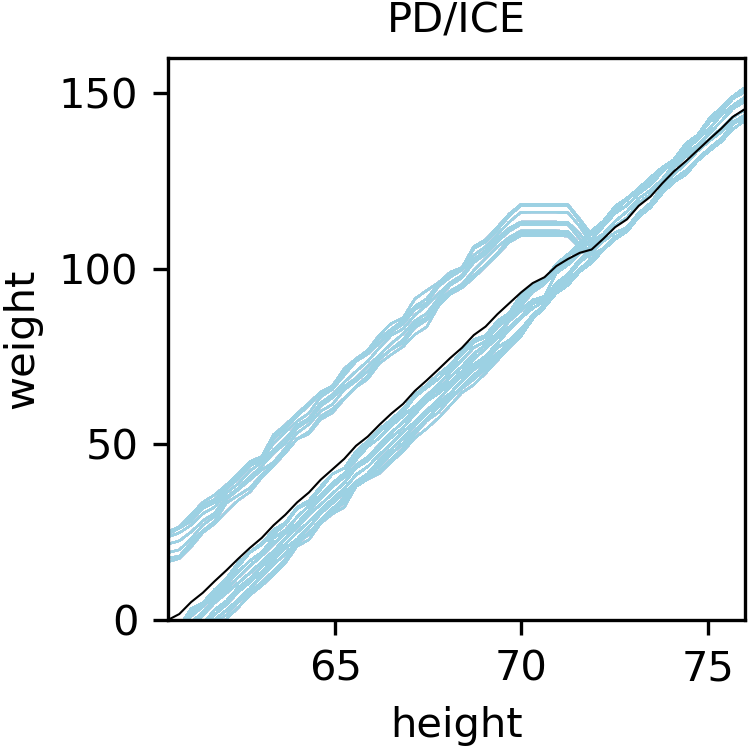
\includegraphics[scale=0.7]{images/height_vs_weight_pdp.png}
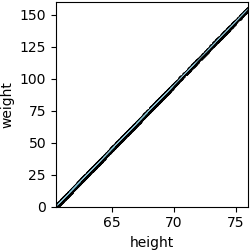
\includegraphics[scale=0.7]{images/height_vs_weight_stratpd.png}
\caption{{\bf  height vs weight}}
\label{fig:height_vs_weight}
\end{center}
\end{figure}

To summarize the hazards of PD and ICE plots, {\em (i)} both are strongly affected by the model chosen by the programmer.  {\em (ii)} To obtain accurate plots, PD and ICE rely on the accuracy of the underlying model, which might sacrifice local accuracy to minimize some global loss function.  Both plots display model prediction results rather than the data itself. {\em (iii)} The potentially inaccurate model feeds off of potentially-nonsensical, synthesized observations arising from variable codependencies. What we need is an accurate mechanism that does not rely on, nor make predictions from, a user's model and a mechanism that does not presume mutually independent features.

\section{Our approach}

In a perfect world, supporting codependent and interacting features would be straightforward because we would know the actual function, $y = f({\bf x})$ or ${\bf y} = f(\bf X)$, that precisely maps a feature vector ${\bf x}_i$ to target value $y_i$ where ${\bf x}_i = ( x_{i1}, .., x_{ip} )$ is a $1 \times p$ row vector of $\bf X$. The partial derivative of $f({\bf x})$ with respect to a variable (column) of interest, $x_c^T = (x_{1c}, .., x_{Nc})$, describes how a unit change in $x_c$ affects $y$ for all $x_c$ values, treating all other variables as constants. Integrating the partial derivative $\frac{\partial}{\partial x_{c}} f({\bf x})$ would yield a curve showing just $x_{c}$'s contribution to $y$. 

Even though $y = f(\bf x)$ is unavailable, a linear regression model, $y = \hat{f}(\bf x)$, provides the general trend of $y$ versus feature $x_c$ via regression coefficient $\beta_c$. For a unit change in $x_c$, $y$ increases or decreases by $\beta_c$, effectively canceling out or controlling for the other features, $x_{(-c)}$, where $x_{(-c)} = x_{j} ~\forall~ j \neq c$. There are a few problems with using a global linear model, however.  First, a linear model might not be strong enough to capture the relationship between all $({\bf x}_i, y_i)$ observation pairs. Second, coefficient $\beta_c$ is a constant and smooths over any local $y$ fluctuations across the entire range of $x_c$. Third, linear models require dummy variables to represent (and replace) categorical $x_c$ variables, therefore, regression coefficients describe the relationship between the presence or absence of a single category and $y$, rather than $x_c$ and $y$.

Another simple but impractical approach stratifies a data set, grouping observations by all features except the feature of interest, $x_c$.  Let $G$ be a group of observations, identified by a set of row indices, where each observation has identical $x_{(-c)}$ features. For a given $G$, the $\{(x_{ic},  y_i)\}_{i \in G}$ pairs then partially describe how $x_c$ affects $y$, all else being equal.  Fitting a univariate linear regressor (without regularization) to group $G$ yields an approximation, $\beta_G$, of the slope of $y$ localized to the specific region of $x_c$ in group $G$; region $R_G = [min(x_{ic}), max(x_{ic})]_{i \in G}$.   Because the $x_c$ regions from multiple groups could overlap, slope $\beta_R$ in any given $x_c$ region, $R$, would be the average of all slope estimates covering that region: $\beta_R = \frac{1}{|G \in R|}\Sigma_{G \in R}\beta_G$. Together, the collection of regions and slopes, $\{(R, \beta_R)\}_{R \in x_c}$, would cover the full $x_c$ range and represent a good localized approximation of the partial derivative of the unknown $f(\bf x)$ with respect to $x_c$.

Alas, this stratification approach works for two or three variables but breaks down for more variables because it is impractical to find groups of observations that are equal across so many variables.  Nonetheless, stratification is simple, well understood, and clearly isolates the effect of $x_c$ on $y$ from the other features for this application, even in the presence of codependent and interacting features.  The only obstacle is a general and practical mechanism for stratifying observations with many variables, which leads us to the primary contribution of this paper.

\subsection{StratPD for numeric variables}

The key idea is to relax stratification so that it organizes observations into groups of similar rather than equal observations.  Our approach, called \spd, uses a CART decision tree \cite{CART} to stratify observations into  groups of similar observations and then collects piecewise linear approximations to the partial derivatives of the unknown $f(\bf x)$ for the groups. Each leaf, $L$, in the tree represents a group with similar $x_{(-c)}$ values and yields a $\beta_L$ from a linear model trained on $(Lx, Ly)$, the $x_c$ and $\bf y$ observations associated with $L$.  The partial derivative between any two (unique and sorted) adjacent $x_c$ data points is estimated by averaging the $\beta_L$ coefficients that overlap that range, yielding $n-1$ partial derivative estimates for $n$ unique $x_c$ values.  Numerically integrating the partial derivatives across $x_c$ space gives a curve representing the contribution of $x_c$ to $y$, as depicted in \figref{fig:leaves}. There are five leaves in \figref{fig:leaves} with regression lines fit through leaf observations, $(Lx, Ly)$. The $x_c$ values in $L_5$ are identical so its infinite slope is ignored.

\begin{figure}[htbp]
\begin{center}
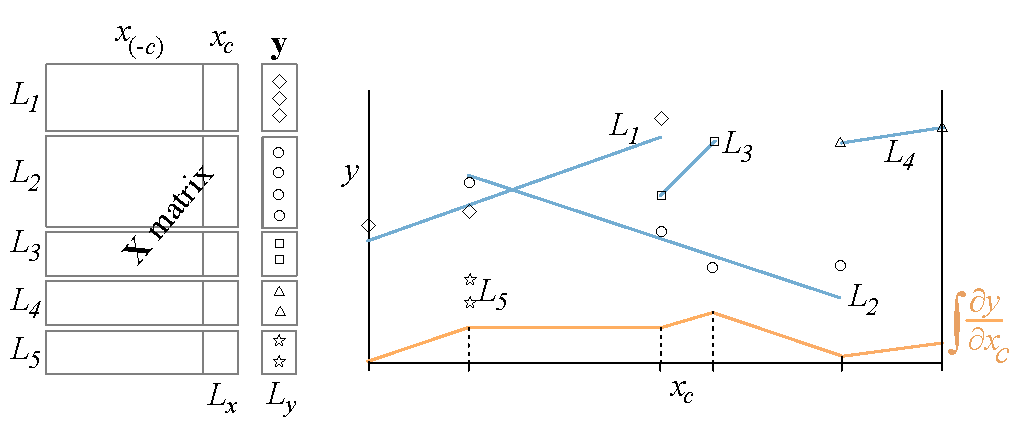
\includegraphics[scale=0.7]{images/leaves.pdf}
\caption{{\bf  Leaves $L_i$...}}
\label{fig:leaves}
\end{center}
\end{figure}

\spd{} trains a decision tree in the usual way but on $(x_{(-c)}, {\bf y})$ rather than $({\bf X}, {\bf y})$. Observations $({\bf x}_{i}, y_i)$ that end up in a tree leaf are, by definition, in the same region of $x_{(-c)}$ feature space. Training greedily partitions feature space in order to minimize variance of $y_i$ within regions, which partitions feature space into tighter and tighter regions.  Tighter regions imply more similar $x_{(-c)}$ values. (The collection of variable inequalities among the decision nodes along the path from from the root to a leaf demarcates the region of feature space.)  The training process must leave at least two samples per leaf in order to fit localized linear models. With too few observations in leaf $L$, $\beta_L$ is a poor estimate; with too many observations, $\beta_L$ is overly-sensitive to contributions from non-$x_c$ features. \spd{} degenerates to a simple marginal plot if training yields a tree with a single leaf node containing all of $x_{(-c)}$.  Algorithm \ref{alg:StratPD} encodes the \spd{} process and the full Python 3 source code is available at {\small \url{https://github.com/parrt/stratpd}}.

Revisiting the \spd{} plot in \figref{fig:height_vs_weight}(d), derived from the apartment rent data set, each blue line represents the regression line with slope $\beta_L$ through the observations in a single leaf of observations with similar $x_{(-c)}$ features. Lines extend from the minimum to maximum $x_c$ value in $L$ ($R_L$). Dropping the $y$-intercept from the regression line effectively erases the contributions of $x_{(-c)}$ features to $Ly$. Because we are interested in the relative contribution of $x_c$ to $y$, \spd{} plots use zero as a $y$-axis baseline. The black dots represent the integration of the partial derivative estimates up to and including each unique $x_c$ value (except the first $x_c$, whose integral value is 0). The partial derivative estimate at an $x_c$ value is the average slope of the blue lines emanating from that value.  

Partial dependence through stratification also works for data sets with categorical variables in $x_{(-c)}$, given a suitable similarity measure between observations that supports categorical variables, but identifying an appropriate categorical similarity measure is a well-known issue.  Decision trees, however, support categorical variables easily and effectively by treating categories as unique integers. Algorithm \ref{alg:StratPD}, therefore, works without modification for $x_{(-c)}$ containing categorical variables. When the column of interest, $x_c$, is categorical, however, a new algorithm is required.

\subsection{StratPD for categorical variables}

The stratification approach can also show how a categorical variable $x_c$ affects $y$, instead of just a single category at a time (if one were forced to one-hot encode $x_c$). As with purely numeric variables, observations with categorical variables that end up in the same leaf are in the same region of feature space. (\todo cite breiman proximity matrix and p595 of ESL book). After stratification by a decision tree trained on $(x_{(-c)}, {\bf y})$, we are left with a regression on a single categorical variable. Because categorical variables can be unordered nominal variables, the notion of $y$ slope is not meaningful between two categories. Instead, the \cspd{} algorithm groups leaf observations $(Lx, Ly)$ by the $Lx$ categories, computes the average $Ly$ value per category, and subtracts $min(Ly)$ to erase the contributions of $x_{(-c)}$.  To get the overall contribution of $x_c$ on $y$ for category $cat$,  \cspd{} averages the leaf contributions for $cat$ across all leaves. See Algorithm \ref{alg:CatStratPD}.

\figref{fig:state_vs_temp}(a) illustrates \spd{} operating on a categorical variable, state, in a synthetic weather data set with data from four states over three years. Temperature data varies in sinusoidal fashion over the year with $N(-5,5)$ noise and different baseline temperatures per state, as the marginal plot in \figref{fig:state_vs_temp}(b) shows. To get the partial dependence of temperature on state, \spd{} stratifies by dayofyear and year then groups similar time buckets by state and computes the average temperature; each blue dot represents a leaf average. The overall temperature estimate per state is the average of those leaf averages, represented by a solid black dash. We use a strip plot to exhibit the variation and density of $y$ values per category. The \spd{} plot accurately identifies the baseline temperature per state, as does the PD/ICE plot in \figref{fig:state_vs_temp}(c).

\begin{figure}[htbp]
\begin{center}
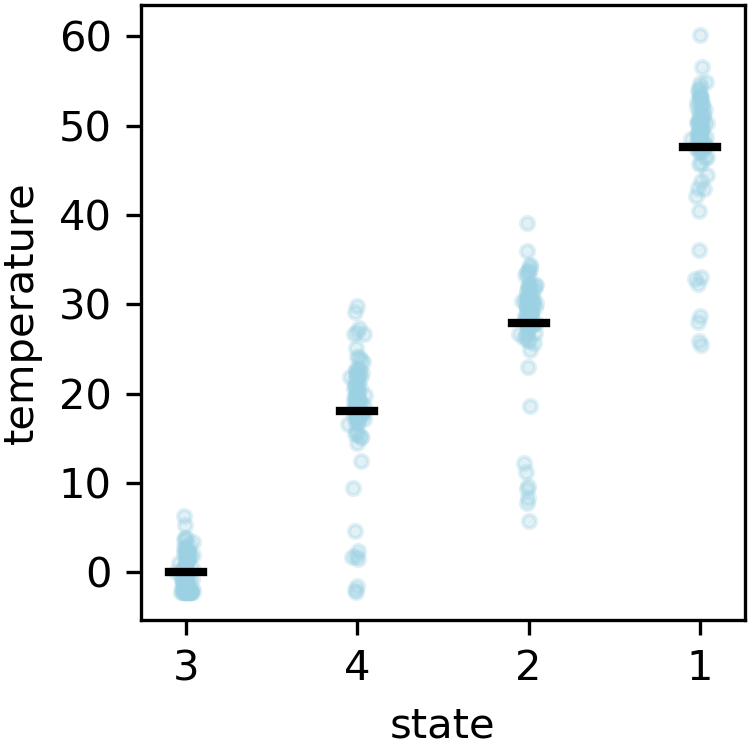
\includegraphics[scale=0.7]{images/state_vs_temp_stratpd.png}
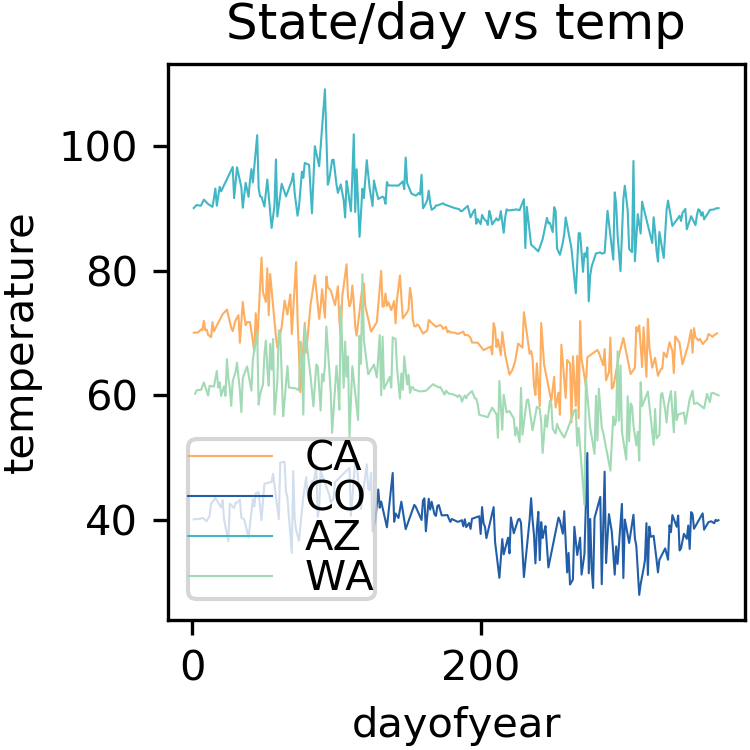
\includegraphics[scale=0.7]{images/dayofyear_vs_temp.png}
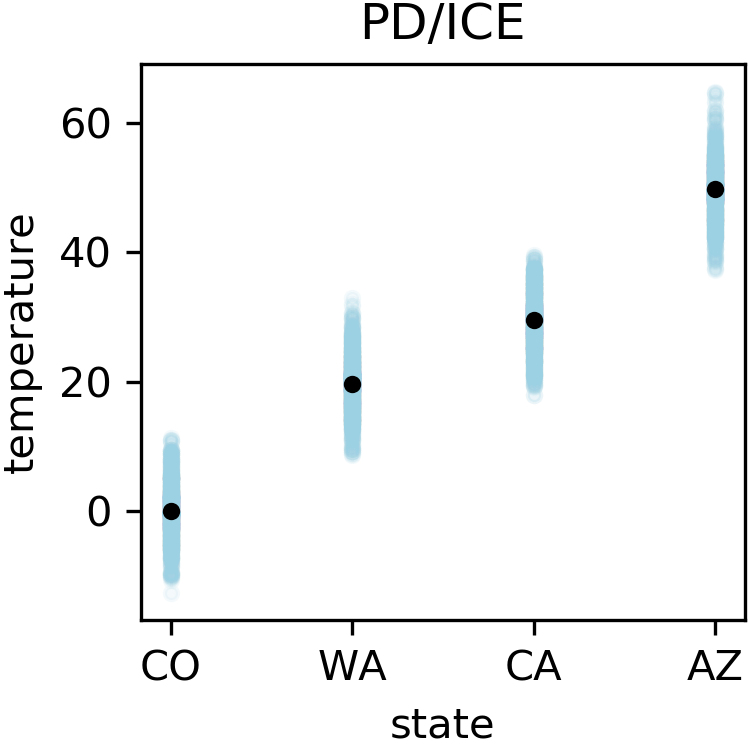
\includegraphics[scale=0.7]{images/state_vs_temp_pdp.png}
\caption{{\bf  state  vs temp}}
\label{fig:state_vs_temp}
\end{center}
\end{figure}

There is a pathological case to consider that can pop up when $x_{(-c)}$ contains a single categorical variable or when the only strongly-predictive variable in $x_{(-c)}$ is categorical.  In this situation, training can yield a decision tree with very large leaves, perhaps hundreds or thousands of observations. Training a single linear model through so many $({\bf x}_i, y_i)$ observations is unlikely to capture the relationship.  The weather data set is a case in point. Choosing  $x_c$=dayofyear, leaves $x_{(-c)}$=\{state,year\} and categorical variable state accounts for most of the variation in target variable temperature.  \figref{fig:dayofyear_vs_temp}(a) shows the marginal plot of state versus temperature. A decision tree splitting on just state, would group all 365 daily temperature observations for a single state into their own leaf. (The marginal plot is showing the complete sine waves but from the side, edge on.)  The \spd{} algorithm described so far would create just four linear models, one per state, and would fail to capture the sine waves. PD and ICE plots, on the other hand, identify the noisy sine waves, as shown in \figref{fig:dayofyear_vs_temp}(b).

pd/ice not smooth

\begin{figure}[htbp]
\begin{center}
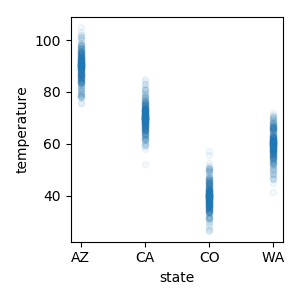
\includegraphics[scale=0.7]{images/state_vs_temp.png}
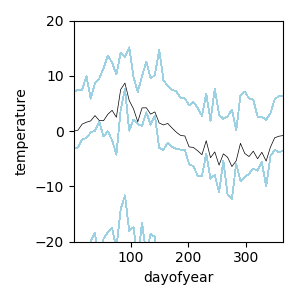
\includegraphics[scale=0.7]{images/dayofyear_vs_temp_pdp.png}
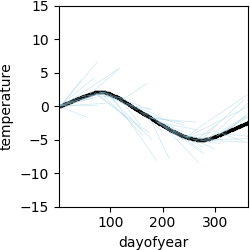
\includegraphics[scale=0.7]{images/dayofyear_vs_temp_stratpd.png}
\caption{{\bf  dayofyear  vs temp}}
\label{fig:dayofyear_vs_temp}
\end{center}
\end{figure}

Pathological case with cat vars: weather sine. lines 6-9 of alg 1.

It's worth mentioning

It's worth examining the role of decision trees

Before moving on, it's worthwhile emphasizing the advantages of stratifying with random forests. Aside from obviating the need to define a similarity measure,

combine derivative in the same plot
categorical variable natively

\subsection{}

\todo{new stuf} y tells us how to partition the feature space into similar groups that are adjacent regions and features space but have similar y. Technically we don't need supervised y but sometimes unsupervised fails, such in the case where p = 2 or p greater than two but with very weak predictors or noise.  The aim is not prediction; instead it is to partition the feature space into similar regions. Consequently we are not worried about over fitting, in fact we wanted to over fit in the sense that it is getting the best partition possible using all the data and all features. Generalization would suffer but we don't care because we want to know about this particular data set. Decision trees mean we don't need to define a similarity measure and we don't need to define been with or another mechanism to draw regions. The regions are optimal to get similar y.

\section{Experimental Results}

effect of sup/unsup: more accurate grouping. ignore noise. unsup fails if p=2 since $x_{(-c)}$ has p=1 and unsup can't distinguish X from synth X.

\todo{add car data}

The data set has an equal number of males and females with $x_{pregnant} \sim U(0,1)$ if female, 65 + $U(-4.5,5)$ if female, and $x_{height} = 68 + U(-7,8)$ if male. 

\[
weight = 120 + 10(x_{height} - min(x_{height})) + 30x_{pregnant} - 1.2x_{education}
\]

\begin{figure}[htbp]
\begin{center}
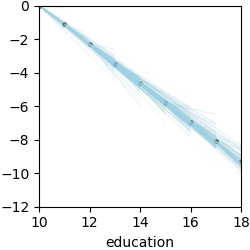
\includegraphics[scale=0.7]{images/education_vs_weight_stratpd.png}
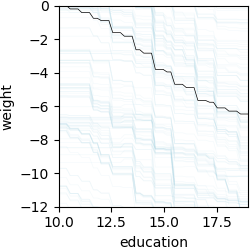
\includegraphics[scale=0.7]{images/education_vs_weight_pdp.png}
\caption{{\bf  Edu vs weight}}
\label{fig:edu_vs_weight}
\end{center}
\end{figure}

\begin{figure}[htbp]
\begin{center}
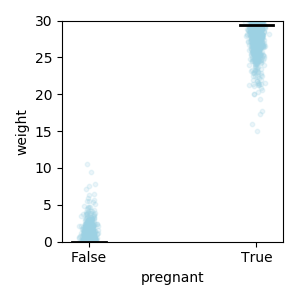
\includegraphics[scale=0.7]{images/pregnant_vs_weight_stratpd.png}
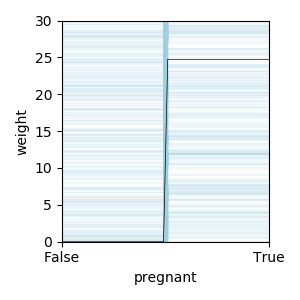
\includegraphics[scale=0.7]{images/pregnant_vs_weight_pdp.png}\\
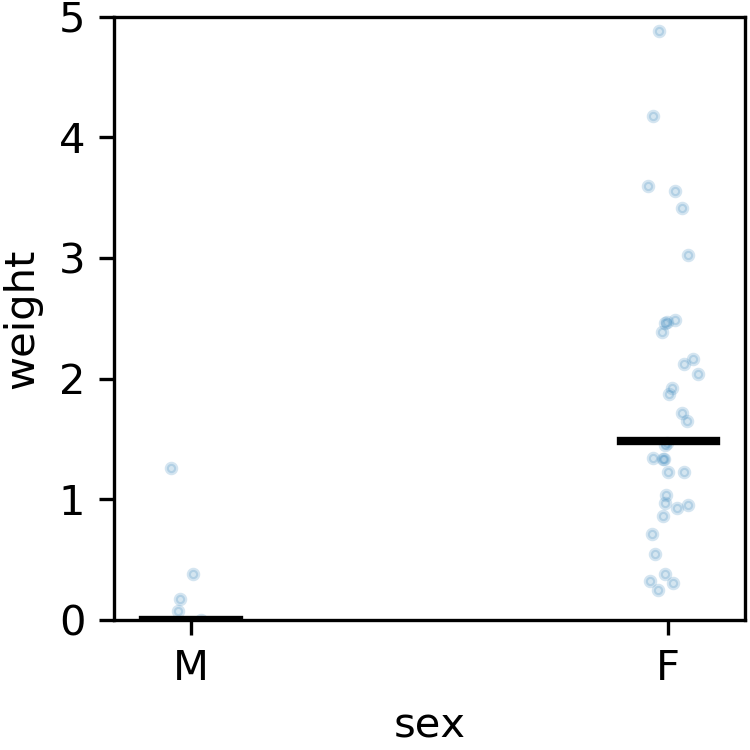
\includegraphics[scale=0.7]{images/sex_vs_weight_stratpd.png}
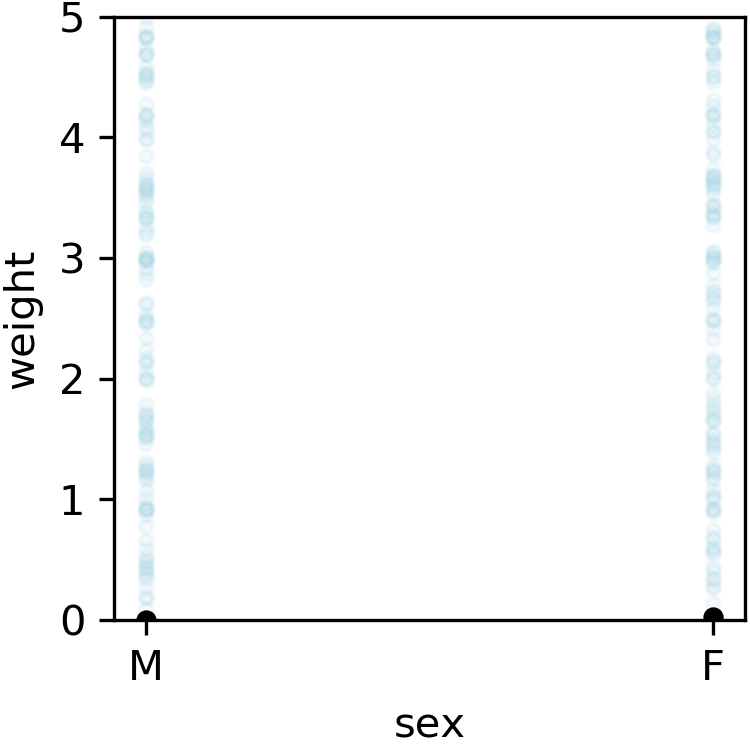
\includegraphics[scale=0.7]{images/sex_vs_weight_pdp.png}
\caption{{\bf  pregnant vs weight}}
\label{fig:pregnant_vs_weight}
\end{center}
\end{figure}


\begin{figure}[htbp]
\begin{center}
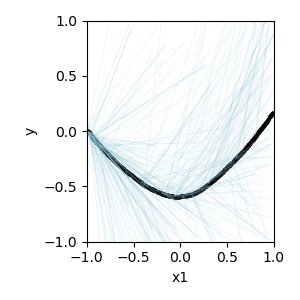
\includegraphics[scale=0.7]{images/add_x1_y_stratpd.png}
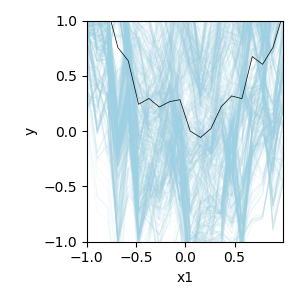
\includegraphics[scale=0.7]{images/add_x1_y_pdp.png}
\\
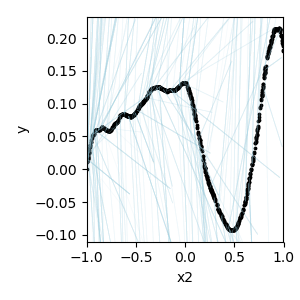
\includegraphics[scale=0.7]{images/add_x2_y_stratpd.png}
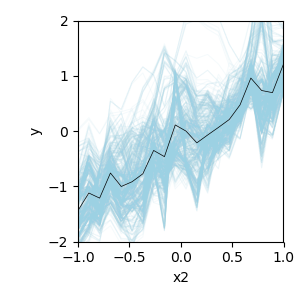
\includegraphics[scale=0.7]{images/add_x2_y_pdp.png}
\caption{{\bf  additive from ICE x1, x2 vs y; $y = x_1^2 + x_2 + \epsilon$, $x_1, x_2, x_3$ are U(-1,1) Sample size 1000}}
\label{fig:add_x1_y_stratpd}
\end{center}
\end{figure}

\begin{figure}[htbp]
\begin{center}
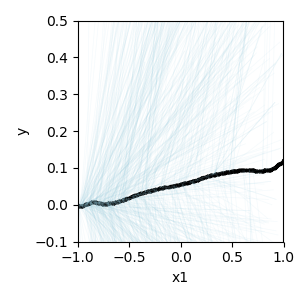
\includegraphics[scale=0.7]{images/bigx_x1_y_stratpd.png}
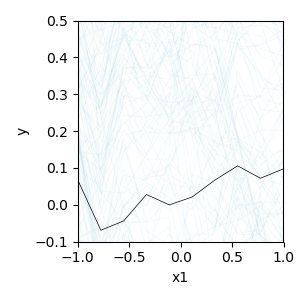
\includegraphics[scale=0.7]{images/bigx_x1_y_pdp.png}
\\
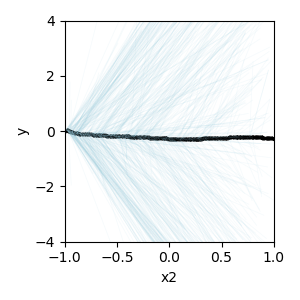
\includegraphics[scale=0.7]{images/bigx_x2_y_stratpd.png}
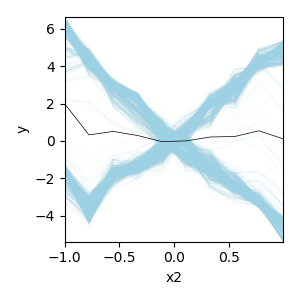
\includegraphics[scale=0.7]{images/bigx_x2_y_pdp.png}
\\
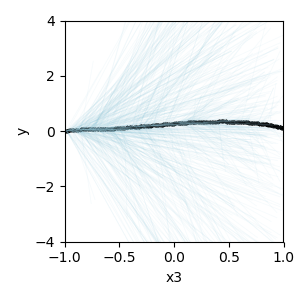
\includegraphics[scale=0.7]{images/bigx_x3_y_stratpd.png}
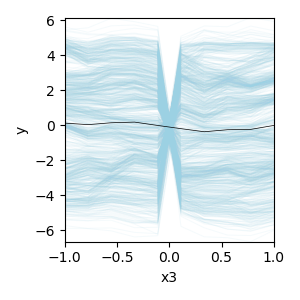
\includegraphics[scale=0.7]{images/bigx_x3_y_pdp.png}
\caption{{\bf  big X from ICE $y = 0.2x_1 - 5x_2 + 10x_2\mathbf{1}_{x_3 \geq 0} + \epsilon$, $x_1, x_2, x_3$ are U(-1,1), Sample size 1000}}
\label{fig:add_x1_y_stratpd}
\end{center}
\end{figure}

\section{Related Work}

There are a few basic approaches to identifying the partial effect of a single variable on the target or response variable:

\begin{itemize}
\item Stratification
\item Beta coefficients from linear model without regularization
\item Marginal plots
\item PDP/ICE
\item Accumulated Local Effects (https://arxiv.org/abs/1612.08468) (ALE) plots
\end{itemize}

PDP math shows that features added or multiplied times the remaining F approximation completely describe the partial dependence; I assume that means that interactions are not a problem.

Most importantly, \spd{} is model-independent in the sense that it does not expect nor rely on a user's model trained on $({\bf X}, {\bf y})$.  \spd{} does, of course, use models internally: a random forest for stratification and multiple linear models for estimating local partial derivatives.  The biggest difference is that \spd{} does not use predictions from any these models, which means prediction accuracy is irrelevant.  (\todo{refer to unsupervised learning trick}.)  In contrast, PD and ICE rely completely on the model supplied by the user and its accuracy.  Some implementations lay a grid across $x_c$'s range and, therefore, potentially make predictions based upon values not present in $x_c$. Also, as discussed, PD and ICE potentially conjure up nonsensical ${\bf }_i$ feature vectors, due to codependencies, and incorporate resulting predictions into plots.

\spd{} was designed to support codependent features, which violates an assumption of PD and ICE. While ICE exposes variable interactions, it is still susceptible to variable codependencies causing misleading plots.

do we need to talk about LIME?

there are other ways to stratify X, such as quartiles or binning of some kind but we have to choose the bins or the similarity measure.

talk about the derivative plot being meaningless in ICE.  they are smoothing and then taking the derivative of suspicious data.
 
propensity stuff James mentioned

talk about how we do not presume independence of features
 
This python package seems to do PDP, LIME etc... https://github.com/oracle/Skater

\section{Future work}

This work describes regressors only, ignoring partial dependence for classifiers.  Research reveals no papers or implementation for classifiers. Friedman, however, briefly describes a partial dependence mechanism for classification whereby $k$-class logistic regression (one-versus-rest) equations indicate the probability of seeing class $k$ at $\bf{x}$.  This suffers from the same interaction-based bias as the regressor model.

better handle on hyper parameters; summarize what we know now.

Actually, the R version of personal dependence may actually do this. See https://christophm.github.io/interpretable-ml-book/pdp.html where he describes PDP for cancer prediction and gets probabilities out.

\section{Conclusion}
\label{sec:conc}

\section{Algorithms}

\setlength{\algomargin}{5pt}
\begin{algorithm}[H]
\label{alg:StratPD}
\LinesNumbered
\SetAlgorithmName{Algorithm}{List of Algorithms}
\SetAlgoSkip{}
\SetInd{.5em}{.5em}
\TitleOfAlgo{{\em StratPD}($X$, $\bf y$, $c$, $hires$=30) {\bf returns} collection of $\beta$ coefficients, $\hat{y}$}
Train random forest regressor {\it rf} on ($x_{(-c)}$, $\bf y$)\\
$leaves$ = leaves(trees({\it rf}))\\
\ForEach{leaf $L \in leaves$}{
	$(Lx, Ly)$ = $\{(x_{ic},  y_i)\}_{i \in L}$\\
	\If{$|L| > hires$}{
		Train random forest regressor {\it rf'} on $(Lx, Ly)$\\
		Add leaves(trees({\it rf'})) to $leaves$\\
	}
	$R_L$ = $[min(Lx), max(Lx)]$\\
	\lIf{left$(R_L)$ = right$(R_r)$}{{\bf continue}}\\
	Fit linear model to $(Lx, Ly)$ giving $\beta_L$\\
}
$uniqx$ = sorted(unique($x_c$))\\
\For{$i=1$ {\bf to} $|uniqx|-1$}{
	$R$ = $(uniqx_i, uniqx_{i+1})$\\
	\ForEach{leaf $L \in {\it rf}$}{
		$\beta_{R} = \frac{1}{|R_L \in R|}\Sigma_{R_L \in R}\beta_L$\\
	}
}
$\hat{y}$ = numerically integrate $\beta_R$'s at $uniqx$\\
\Return{collection of all $\beta_R$ and $\hat{y}$}
\end{algorithm}

\setlength{\algomargin}{5pt}
\begin{algorithm}[H]
\label{alg:CatStratPD}
\LinesNumbered
\SetAlgorithmName{Algorithm}{List of Algorithms}
\SetAlgoSkip{}
\SetInd{.5em}{.5em}
\TitleOfAlgo{{\em CatStratPD}($X$, $\bf y$, $c$) {\bf returns} dictionary mapping category to effect on $y$}
Train random forest regressor {\it rf} on ($x_{(-c)}$, $\bf y$)\\
Let $D$ be dictionary mapping category to $y$ value\\
\ForEach{leaf $L \in {\it rf}$}{
	$(Lx, Ly)$ = $\{(x_{ic},  y_i)\}_{i \in L}$\\
	\ForEach{$cat \in Lx$}{
		$cat_y$ = $Ly[Lx=cat]$\\
		\lIf{$|cat_y| < 2$}{{\bf continue}}\\
		$cat_{avg}$ = $\frac{1}{|cat_y|} \Sigma cat_y$\\
		$cat_{avg}$ = $cat_{avg} - min(Ly)$\tcp*[r]{\it Strip y contribution from $x_{(-c)}$}
		$D_{cat}$ = $D_{cat} + cat_{avg}$\\
	}
}
Let $n_{cat}$ be number of $cat_{avg}$ added to $D_{cat}$\\
$D_{cat}$ = $D_{cat} / n_{cat}$\tcp*[r]{\it Take average of leaf averages for $cat$}
\Return{$D_{cat}$}
\end{algorithm}

\bibliographystyle{apalike}

\bibliography{stratpd}
\end{document}